\chapter{Cómo se metió el Tarot 650 en Gazebo}

\begin{enpocas}
Cómo se pasó el dron de un archivo CAD a un modelo que vuela en Gazebo: las mallas, la tabla de parámetros, los motores, el mezclador, los sensores y el viento.
\end{enpocas}

\begin{figure}[H]
\centering
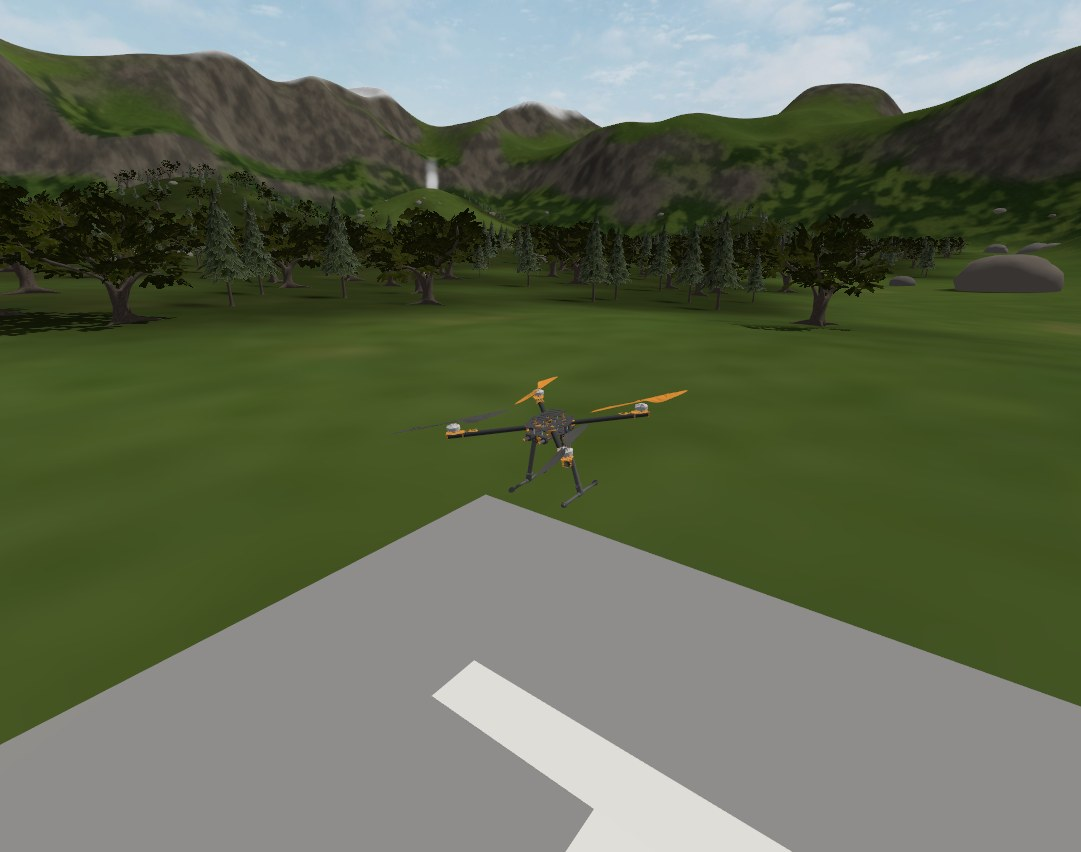
\includegraphics[width=0.78\textwidth]{gz_tarot_cerca.jpg}
\caption{El Tarot 650 en vuelo estacionario sobre la base de despegue del mundo
\cod{bosque_grande}. Las hélices delanteras son naranjas.}
\label{fig:tarot-gz}
\end{figure}

\section{Del CAD a las mallas}

La geometría viene del modelo de GrabCAD \emph{Tarot Ironman 650}
(\url{https://grabcad.com/library/tarot-ironman-650-2}), con motores T-Motor MN3508 y hélices
de $15\times5$''. El archivo \cod{Tarot.stp} es un ensamble de cientos de piezas. Se convirtió
con \cod{scripts/cad_a_malla.py} en dos pasos:

\begin{lstlisting}[style=bash]
# 1) Ver las piezas: nombre, cuántas hay y su tamaño
~/.venvs/cad/bin/python scripts/cad_a_malla.py listar "Tarot 650/Tarot.stp"

# 2) Exportar grupos de piezas por nombre (expresiones regulares)
~/.venvs/cad/bin/python scripts/cad_a_malla.py exportar "Tarot 650/Tarot.stp" salida/ \
    --grupo placas='Base$|base|side bracket|lower support|bracket landing' \
    --grupo brazos='CarbonArm' \
    --grupo acentos='orange|clamp|pivot|clip|Motortoarm|ArmCopter|cap' \
    --grupo tren='Lower Tube|leg|foot|landing-gear|Landing' --grupo motores='bell' \
    --grupo marco=resto --excluir '94180|bearing|circlip|coil|axle|stator|15x5' \
    --ejes +z +x +y --origen 0.0142 0 0.0070

# Hélices, cada una por aparte y centrada:
~/.venvs/cad/bin/python scripts/cad_a_malla.py exportar "Tarot 650/Tarot.stp" salida/ \
    --grupo helice='15x5' --separar helice --caras 4000 --ejes +z +x +y --origen 0.0142 0 0.0070
\end{lstlisting}

\begin{itemize}
  \item \cod{--ejes +z +x +y} dice qué eje del CAD es el \emph{x} (frente), el \emph{y}
        (izquierda) y el \emph{z} (arriba) del modelo. El frente quedó paralelo a los patines del
        tren de aterrizaje.
  \item \cod{--origen} es el punto del CAD (en metros) que queda en el origen del cuerpo.
  \item Cada grupo se exporta como un STL con su color en el SDF: placas y brazos de carbono,
        acentos naranjas, tren, campanas de los motores y el resto del marco.
  \item \cod{helice_i.stl} se asigna al rotor $i$ por su posición.
\end{itemize}

\begin{aviso}
No se deben simplificar \cod{placas} ni \cod{brazos}: las placas de carbono miden 1.6~mm y la
simplificación de la malla las deshace. Sí se pueden reducir \cod{acentos} (50\,000 caras),
\cod{tren} (25\,000) y \cod{motores} (20\,000).
\end{aviso}

\begin{figure}[H]
\centering
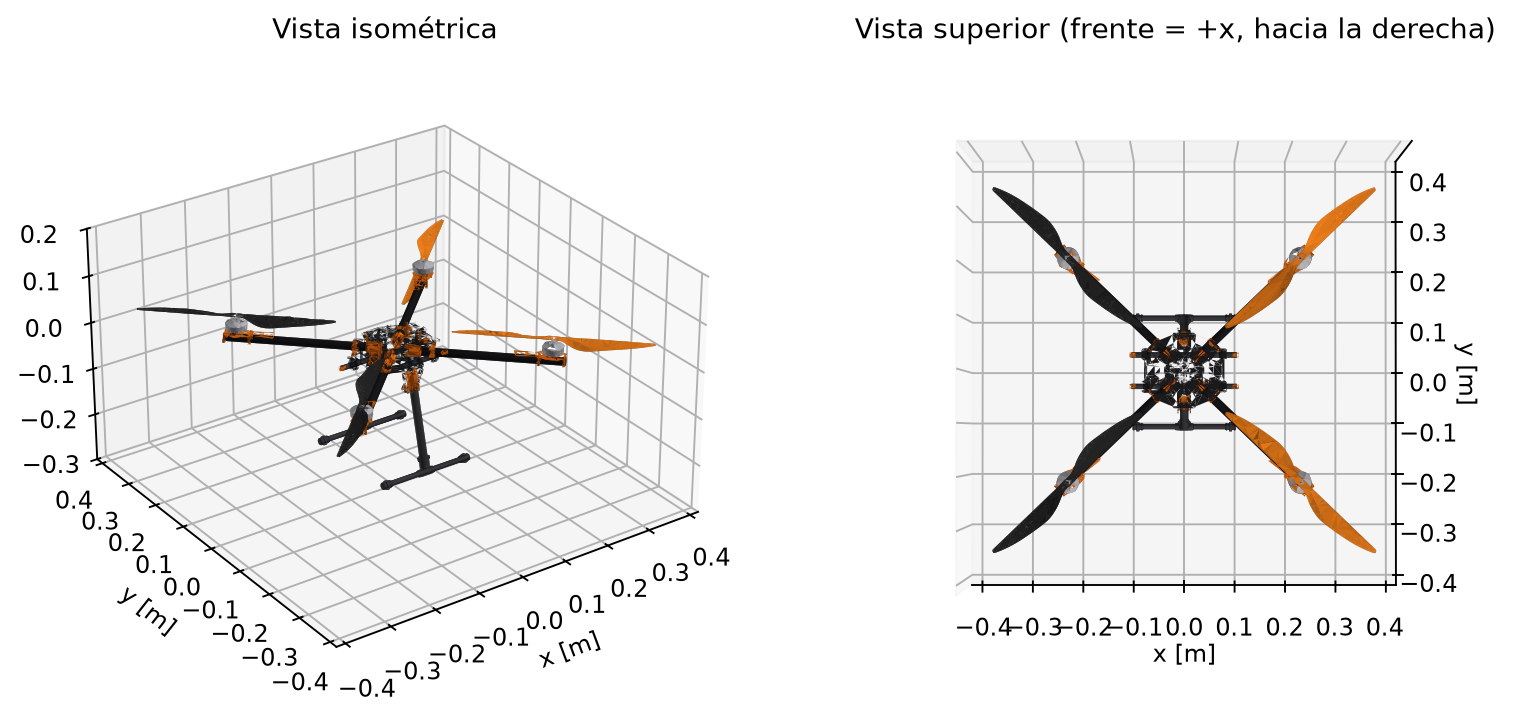
\includegraphics[width=\textwidth]{tarot_render.png}
\caption{Mallas del Tarot convertidas del CAD (\cod{models/tarot650/meshes}), en el marco del
cuerpo.}
\end{figure}

\section{Parámetros del vehículo}

Todos los parámetros están en una sola tabla, \cod{VEHICULOS} de \cod{scripts/generar_modelo.py}.
De ella salen la planta que simula Gazebo (\cod{models/tarot650/model.sdf}) y los valores que usa
el controlador (\cod{config/vehiculo_tarot650.yaml}), así que el modelo del controlador coincide
siempre con la planta. Para cambiar un parámetro se edita la tabla y se vuelve a correr:

\begin{lstlisting}[style=bash]
python3 scripts/generar_modelo.py            # todos los vehículos
python3 scripts/generar_modelo.py tarot650   # solo uno
\end{lstlisting}

\begin{table}[H]
\centering\small
\begin{tabular}{lll}
\toprule
\textbf{Parámetro} & \textbf{Valor} & \textbf{Origen} \\ \midrule
Configuración & ``X'', 4 rotores & CAD \\
Posición de los rotores $(x_i, y_i)$ & $(\pm0.2198,\ \pm0.212)$~m & CAD \\
Altura de los rotores & 0.04~m sobre el origen & CAD \\
Tren de aterrizaje & dos patines a lo largo de \emph{x}, 0.2205~m bajo el origen & CAD \\
Radio de la hélice & 0.1905~m (15'') & CAD \\
Masa total & 2.2~kg (cuerpo 2.12 + 4 rotores de 0.02) & supuesto \\
Inercia total $J$ & diag(0.03412, 0.03609, 0.06596)~kg\,m$^2$ & estimada \\
Constante de empuje $k_f$ & $4.24\times10^{-5}$~N/(rad/s)$^2$ & supuesto \\
Constante de par $k_m$ & 0.016~m & supuesto \\
Velocidad máxima $\omega_{max}$ & 680~rad/s ($\approx$ 19.6~N por motor) & supuesto \\
Constante de tiempo del motor & 30~ms al subir, 50~ms al bajar & supuesto \\
Velocidad en vuelo estacionario & 357~rad/s & calculada \\
Lazo de actitud $K_R$, $K_\omega$ & (3.4, 3.6, 1.65), (0.55, 0.58, 0.59) & ajustado \\
Cámara & 640$\times$480, 15~Hz, HFOV 1.3~rad, 30° hacia abajo & diseño \\
LiDAR 3D & 360°$\times$120 haces, 16 canales ($-35^\circ$ a $+15^\circ$), 30~m, 10~Hz & diseño \\
\bottomrule
\end{tabular}
\caption{Parámetros del Tarot 650 en la simulación.}
\label{tab:tarot}
\end{table}

\begin{aviso}
La geometría es la del CAD, pero la masa, las inercias, $k_f$, $k_m$ y los retardos son valores
típicos supuestos para esta configuración. \textbf{Hay que reemplazarlos por los del dron real}
(peso con batería, KV de los motores, hélice, número de celdas) antes de sacar conclusiones
cuantitativas.
\end{aviso}

\section{Motores y mezclador}

Cada rotor es un \cod{MulticopterMotorModel} de Gazebo: recibe una velocidad de referencia
(\cod{/cuadrirotor/command/motor_speed}, un mensaje \cod{Actuators} con las cuatro velocidades),
la filtra con un sistema de primer orden y produce el empuje $f_i = k_f\,\omega_i^2$ y el par de
arrastre $k_m f_i$. Fragmento del SDF generado para el rotor 0:

\begin{lstlisting}[style=xml]
<plugin filename="gz-sim-multicopter-motor-model-system"
        name="gz::sim::systems::MulticopterMotorModel">
  <robotNamespace>cuadrirotor</robotNamespace>
  <jointName>rotor_0_joint</jointName>
  <linkName>rotor_0</linkName>
  <turningDirection>ccw</turningDirection>
  <timeConstantUp>0.03</timeConstantUp>
  <timeConstantDown>0.05</timeConstantDown>
  <maxRotVelocity>680.0</maxRotVelocity>
  <motorConstant>4.24e-05</motorConstant>
  <momentConstant>0.016</momentConstant>
  <commandSubTopic>command/motor_speed</commandSubTopic>
  <motorNumber>0</motorNumber>
  <rotorDragCoefficient>8.06428e-05</rotorDragCoefficient>
  <rollingMomentCoefficient>1e-06</rollingMomentCoefficient>
  <motorSpeedPubTopic>motor_speed/0</motorSpeedPubTopic>
  <rotorVelocitySlowdownSim>10</rotorVelocitySlowdownSim>
  <motorType>velocity</motorType>
</plugin>
\end{lstlisting}

\begin{figure}[H]
\centering
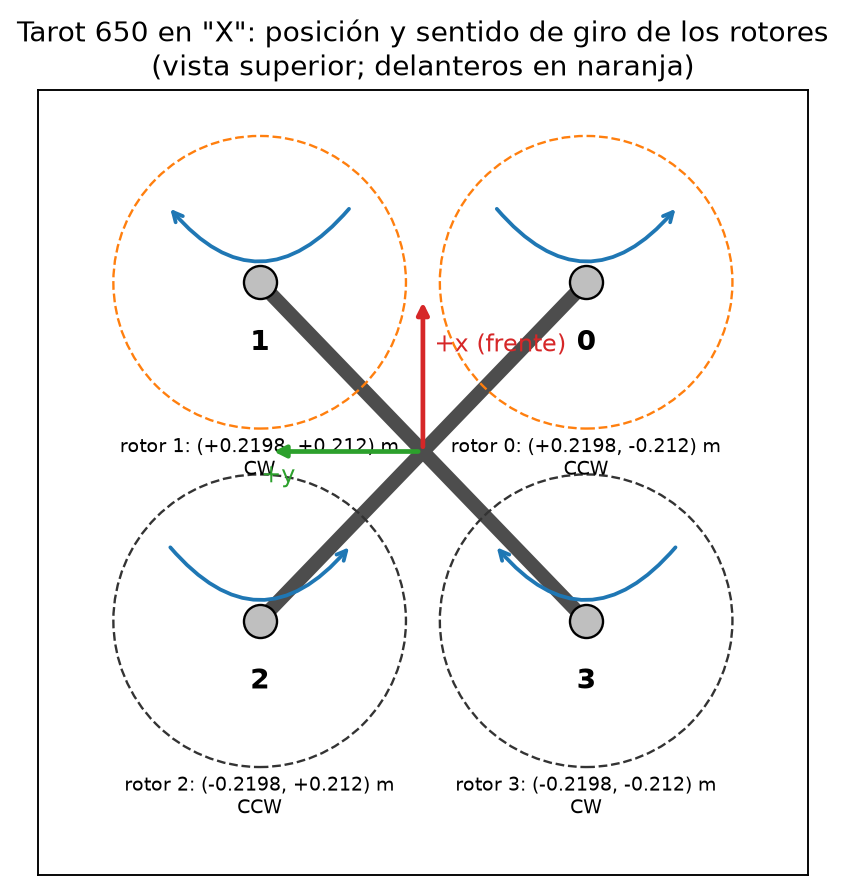
\includegraphics[width=0.62\textwidth]{tarot_planta.png}
\caption{Numeración, posición y sentido de giro de los rotores del Tarot.}
\label{fig:planta}
\end{figure}

El controlador calcula un empuje total $T$ y un par $\tau=(\tau_x,\tau_y,\tau_z)$. El mezclador
(\cod{dinamica.Mezclador}) los convierte en velocidades de rotor. Con el rotor $i$ en
$(x_i,y_i)$ y sentido $s_i$ ($+1$ antihorario, $-1$ horario):
\begin{equation}
\begin{bmatrix} T\\ \tau_x\\ \tau_y\\ \tau_z \end{bmatrix} =
\underbrace{\begin{bmatrix}
1 & 1 & 1 & 1\\
y_0 & y_1 & y_2 & y_3\\
-x_0 & -x_1 & -x_2 & -x_3\\
-s_0 k_m & -s_1 k_m & -s_2 k_m & -s_3 k_m
\end{bmatrix}}_{B}
\begin{bmatrix} f_0\\ f_1\\ f_2\\ f_3 \end{bmatrix},
\qquad
\omega_i = \sqrt{\frac{\operatorname{sat}_{[0,\,f_{max}]}\big((B^{+}[T,\tau]^\top)_i\big)}{k_f}} .
\end{equation}

En vuelo estacionario cada motor carga un cuarto del peso:
\begin{equation}
f_h = \frac{mg}{4} = \frac{2.2\cdot 9.81}{4} = 5.40\ \text{N},\qquad
\omega_h = \sqrt{\frac{f_h}{k_f}} = 357\ \text{rad/s},\qquad
\frac{f_h}{f_{max}} = \Big(\frac{357}{680}\Big)^2 = 0.28 .
\end{equation}
La relación empuje/peso es $4\cdot19.6/21.6\approx3.6$.

\begin{figure}[H]
\centering
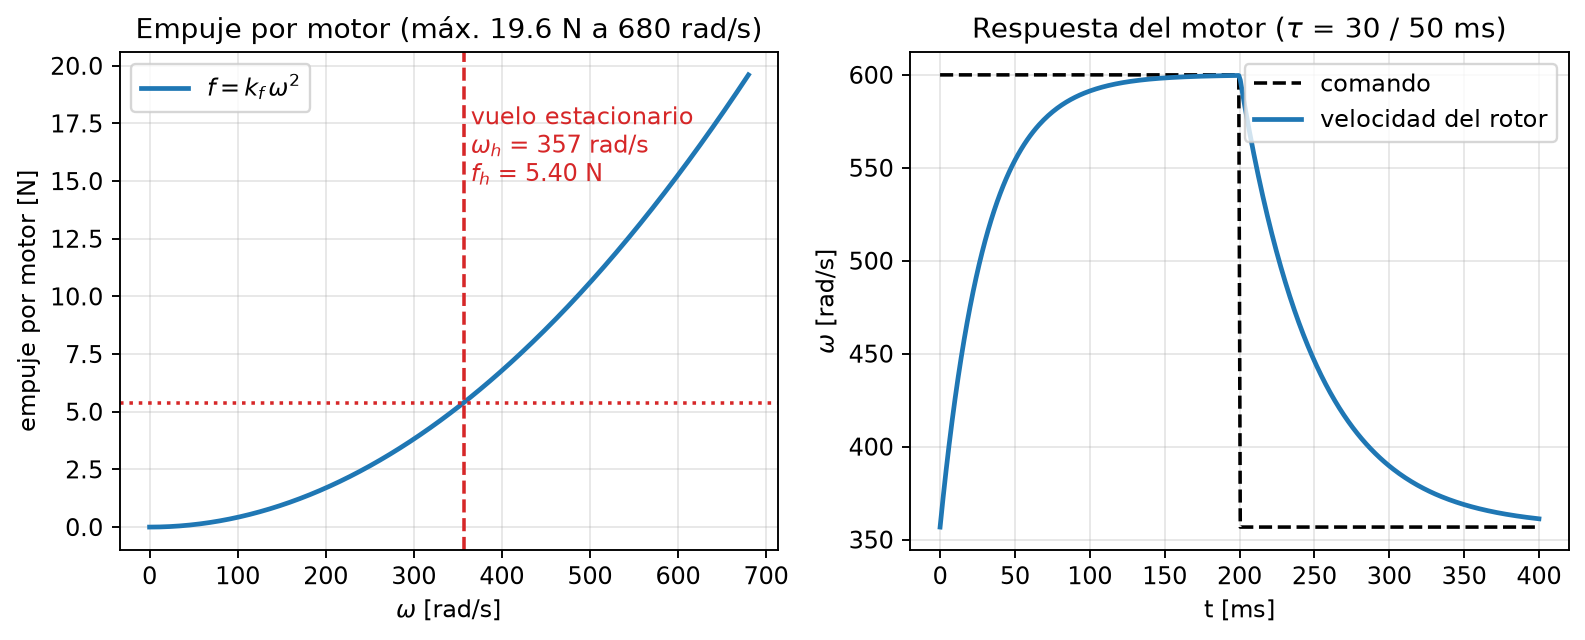
\includegraphics[width=\textwidth]{motor_empuje.png}
\caption{Curva de empuje de un motor y respuesta de primer orden a un escalón.}
\end{figure}

\section{Sensores}

\begin{description}
  \item[IMU] 200~Hz en \cod{/cuadrirotor/imu}.
  \item[Odometría] \cod{OdometryPublisher} a 1~kHz en \cod{/cuadrirotor/odometria} (posición y
        orientación verdaderas; velocidades en el marco del cuerpo).
  \item[Cámara frontal] inclinada 30° hacia abajo: ve el horizonte para buscar el humo de lejos y
        mantiene el foco a la vista en la órbita. Rango de recorte hasta 1500~m (antes 200~m) para
        que se vean las montañas.
  \item[LiDAR 3D] para la evasión de obstáculos (capítulo~\ref{cap:autonomia}):
\end{description}

\begin{lstlisting}[style=xml]
<sensor name="lidar" type="gpu_lidar">
  <pose>0 0 0.1 0 0 0</pose>
  <always_on>1</always_on>
  <update_rate>10</update_rate>
  <topic>cuadrirotor/lidar</topic>
  <lidar>
    <scan>
      <horizontal><samples>120</samples><min_angle>-3.14159</min_angle><max_angle>3.14159</max_angle></horizontal>
      <vertical><samples>16</samples><min_angle>-0.6109</min_angle><max_angle>0.2618</max_angle></vertical>
    </scan>
    <range><min>0.8</min><max>30</max><resolution>0.05</resolution></range>
  </lidar>
</sensor>
\end{lstlisting}

El alcance mínimo de 0.8~m evita que el LiDAR vea las propias hélices (las puntas quedan a
$\approx$0.5~m del centro). La nube llega a ROS como \cod{sensor_msgs/PointCloud2} en
\cod{/cuadrirotor/lidar/points}.

\section{Perturbación de viento}

El sistema \cod{FuerzaViento} (\cod{cuadrirotor_gz_plugins}) aplica sobre \cod{base_link} una fuerza
en el marco inercial y la mantiene en cada paso de física hasta que llega un valor nuevo; así la
perturbación es exactamente la señal publicada, sin acumularse. El nodo \cod{viento} publica
\begin{equation}
F(t) = F_0 + A\sin(2\pi f t),\qquad F_0 = 1\ \text{N},\ A = 0.5\ \text{N},\ f = 0.2\ \text{Hz},
\end{equation}
a partir de $t = 15$~s (con \cod{viento:=true}).
